\chapter{Bildverarbeitung und Umsetzung}
\label{cha:verarbeitungumsetzung}

Zusammenfassend l"asst sich der Ablauf unseres Programms,
das das Problem der Lokalisierung eines Helikopters im Raum l"ost, folgenderma"sen beschreiben:\newline
Anfangs werden die Kameras separat kalibriert. Ist der berechnete Fehler dieser Kalibrierung gering, werden anschlie"send die Kameras zueinander kalibriert. Wird dann mit beiden Kameras ein Bild der Szene aufgenommen, werden diese Bilder zuerst rektifiziert und anschlie"send entzeichnet. Mit den neuen Bildern ist es m"oglich, eine Tiefenkarte und anschlie"send eine Punktewolke zu generieren. Von dieser Punktewolke wird dann der Mittelpunkt und dessen Koordinaten bestimmt, welche der Position des Helikopters entsprechen.\newline
Diese Schritte werden im Folgenden detailliert beschrieben.

\section{Kalibrierung}
\label{sec:kalibrierung}

F"ur eine Messung, bei der der Fehler minimiert werden soll, ist das Kalibrieren der Kameras unumg"anglich. Durch die Linse einer Kamera entsteht eine tonnenf"ormige Verzeichnung. Diese Fehler sind meist so klein, dass sie vom menschlichen Auge nicht erfasst werden k"onnen \cite{VZ} \cite{VZ1}. Durch die Kalibrierung der Kamera k"onnen diese kompensiert werden.\newline

\begin{figure}[H]
	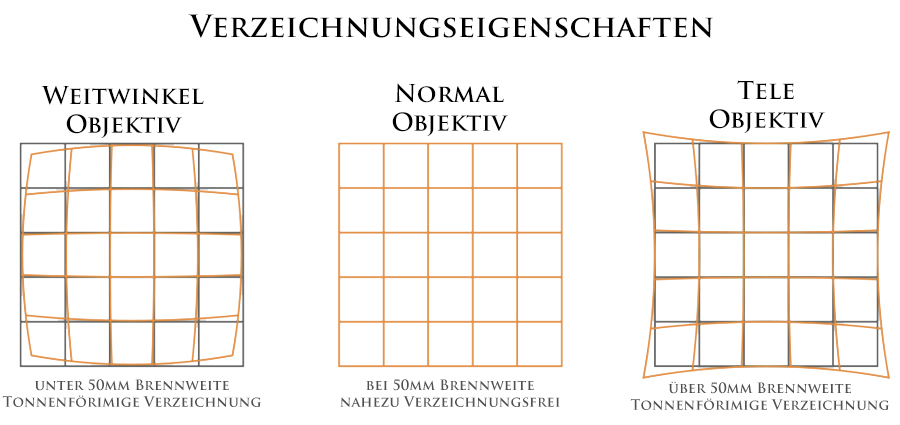
\includegraphics[scale=0.45]{bilder/verzeichnung}
	\caption[Verzeichnung]{Verzeichnung}
	\label{fig:verzeichnung}
	\small  uelle: \url{http://www.fotokurs-bremen.de/wp-content/uploads/2016/11/Objektiv-Verzeichnung.jpg}
\end{figure}

\noindent Durch die Kamerakalibrierung werden folgende Parameter bestimmt:

\begin{description}
	\item[Intrinsische Parameter]
	Bezeichnen die Abbildung von 3D-Punkten im Kamerakoordinatensystem auf den 2D-Sensor der Kamera. Es sind Informationen der Kamera selbst, die unabh"angig davon sind, wo sich die Kamera befindet und wie diese ausgerichtet ist.
	
	\item[Extrinsische Parameter]
	Die r"aumliche Lage und Orientierung, d.h. Translation und Rotation der Kamera zu einem Referenzkoordinatensystem \cite{cal} \cite{extr}.
\end{description}

\noindent Da es ich bei dem System um ein Stereokamera-System handelt, ist die Kalibrierung von diesem etwas komplizierter.\newline
Zuerst m"ussen die Kameras gesondert kalibriert werden. Dies wird mit der Funktion \textit{calibrateCamera} von OpenCV durchgef"uhrt. F"ur die Kalibrierung wird ein Schachbrett-Muster verwendet. Wichtig ist, dass bei der Kalibrierung von Stereokameras dasselbe Bild verwenden. F"ur die Erkennung der Eckpunkte des Schachbretts wird die OpenCV-Funktion \textit{findChessboardCorners} verwendet. Diese liefert die Objekt- und Bild-Punkte der Aufnahme. Bei den Objekt-Punkten handelt es sich um die 3D-Punkte des Bildes, bei den Bild-Punkten um die 2D-Punkte \cite{OcvD}. In \ref{fig:chessboards} sieht man das Resultat von \textit{findChessboardCorners}. Die gefundenen Ecken des Schachbretts werden hier farblich visualisiert.

\begin{figure}[H]
	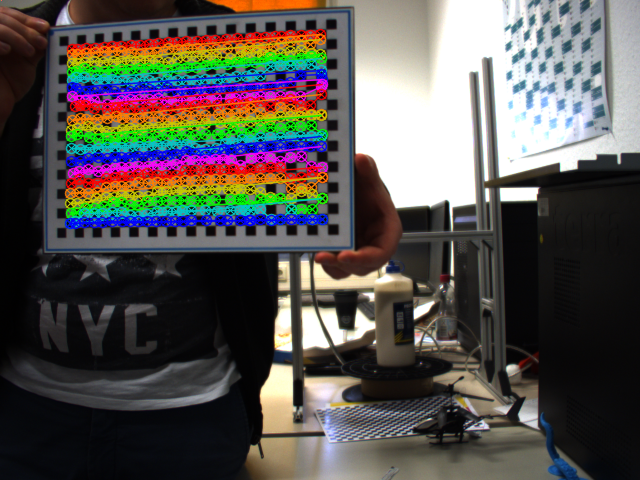
\includegraphics[scale=0.4]{bilder/calibration}
	\caption[Kalibrierung]{Kalibrierung}
	\label{fig:chessboards}
\end{figure}

\noindent F"ur eine m"oglichst genaue Kalibrierung werden 50 Bilder verwendet. Anhand dieser wird jede Kamera mittels \textit{calibrateCamera} kalibriert.\newline
Die Funktion liefert die intrinsisches Parameter in Form von einer \textit{3 x 3} Kamera-Matrix.

\begin{figure}[H]
	\centering
	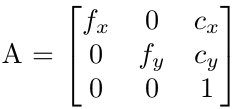
\includegraphics[scale=0.75]{bilder/matrix}
\end{figure}

\noindent Wobei $f_{x}$ und $f_{y}$ die Brennweite in Pixeln und $c_{x}$ $c_{y}$ der Hauptpunkt, der normalerweise in der Bildmitte liegt, ist.

\noindent Die Ergebnisse dieses Vorgangs werden auf dem Computer gespeichert, sodass dieser nicht wiederholt werden muss. Anschlie"send wird das Ergebnis der Kalibrierungen an die OpenCV-Funktion \textit{stereoCalibrate} "ubergeben.\newline
Mit Hilfe der Stereo-Kalibrierung kann der Zusammenhang zwischen den Kameras ermittelt werden: Es werden von dem Bezugsbild, welches zum Ursprung des Koordinatensystems wird, die Objekt-Punkte verwendet. Von beiden Kamerasystemen werden die Bild-Punkte, die jeweiligen Kameramatrizen und die Verzeichnungskoeffizienten verwendet. Die f"ur uns wichtigsten Ergebnisse der Stereo-Kalibrierung sind die Rotation und Translation der beiden Kameras zueinander.

\section{Genauigkeitsabsch"atzung der Kalibrierung}
\label{sec:fehlertest}

Der Reprojection Error ist ein qualitatives Ma"s für die Genauigkeit. Der Reprojection Error ist die Distanz zwischen einem detektierten Punkt in dem kalibrierten Bild und dem korrespondierendem Weltpunkt projiziert in dasselbe Bild. Die Reprojection Error Methode ist ein Diagnosewerkzeug um zu erkennen ob eine Verbesserung der Kalibrierung n"otig ist oder nicht. Dies wird in \ref{fig:repro} visuell dargestellt.

\begin{figure}[H]
	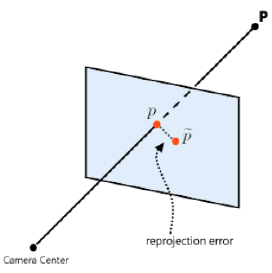
\includegraphics[scale=0.75]{bilder/repro_error}
	\caption[Reprojection Error]{Reprojection Error}
	\label{fig:repro}%
	\small Quelle: \url{https://www.researchgate.net/figure/The-reprojection-error-is-the-distance-between-the-projected-image-point-p-and-the_fig3_267557759}
\end{figure}

\section{Stereokalibrierung}
\label{sec:stereokalibrierung}

\begin{figure}%
	\centering
	\subfloat[Stereosystem]{{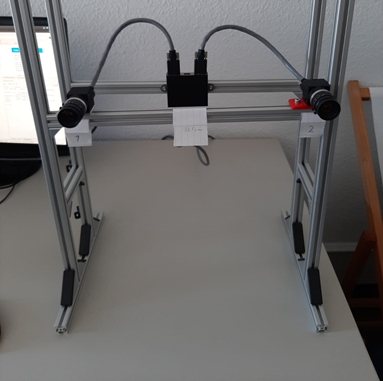
\includegraphics[width=6cm]{bilder/camerasystem} }}%
	\qquad
	\subfloat[Szenenaufnahme]{{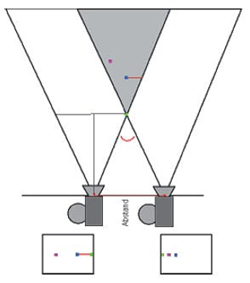
\includegraphics[width=6cm]{bilder/szene} }}%
	\caption{Stereo-System}%
	\small Quelle: \url{https://me.efi.th-nuernberg.de/interaktion/index.php5/Bearbeitung_und_Gewinnung_von_Tiefeninformation_durch_die_Kopplung_zweier_Kameras}
	\label{fig:stereo1}%
\end{figure}

Wie auf dem Bild \ref{fig:stereo1} zu sehen ist, handelt es sich bei unserem Aufbau um ein Stereosystem. Die beiden Kameras sind horizontal zueinander verschoben, fotografieren aber zum gr"o"sten Teil die selbe Szene. Dies ist notwendig f"ur das Berechnen von Tiefeinformationen. Liegen alle Referenzpunkte auf einer Geraden, so kann mittels Triangulation, wie auf \ref{fig:baseline} zu sehen ist, der $z$-Achsen Wert der Punkte berechnet werden.

\begin{figure}[H]
	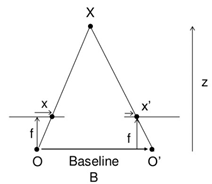
\includegraphics[scale=1.5]{bilder/baseline}
	\caption[Z-Achsen Berechnung]{Z-Achsen Berechnung}
	\label{fig:baseline}%
	\small Quelle: \url{https://opencv-python-tutroals.readthedocs.io/en/latest/py_tutorials/py_calib3d/py_depthmap/py_depthmap.html}
\end{figure}

\noindent Da die Kameras nur horizontal verschoben sind, erhalten wir den Stereonormalfall, der wie folgt beschrieben wird: \textit{Das achsparallele Stereosystem zeichnet sich durch zwei Kameras aus, die nur horizontal verschoben und deren Koordinatensysteme nicht gegeneinander verdreht sind \cite{Tu}.} \newline
\noindent Bei der Stereokalibrierung werden sowohl die inneren Kameraparameter f"ur das Stereokamerapaar, als auch die geometrische Lage zwischen den Kameras berechnet \cite{zbs}. OpenCV bietet hierf"ur die Funktion \textit{stereoCalibrate}. Diese Funktion erwartet die vorher berechneten Kameramatrizen und Verzeichnungskoeffizienten beider Kameras. Zudem werden von beiden Kameras Bildpunkte ben"otigt, die auf die selben Objektpunkte abbilden. Demnach m"ussen beide Kameras auf das selbe Kalibrierobjekt kalibriert werden \cite{ocvs}. Im Programm wird mit beiden Kameras ein Foto der Szene gemacht und anschlie"send versucht, das Schachbrettmuster zu detektieren. War die Detektion bei beiden Bildern erfolgreich, werden die Bild- und Objekt-Punkte gespeichert und der Vorgang 50 mal wiederholt. Nach 50 erfolgreichen Detektionen werden die Kameras zueinander kalibriert.\newline
Durch die Stereokalibrierung erhalten wir die Rotation und Translation beider Kameras zueinander. Mit diesen Werten ist es m"oglich, Informationen zur Tiefe zu ermitteln.

\subsection{Entzeichnung}
\label{sec:entzeichnung}

Durch das Objektiv einer Kamera entstehen bei der optischen Abbildung Verzeichnungen. Die Stärke dieser ist dabei vom eingesetzten Objektiv abhängig \cite{wie}. Die Verzerrung sorgt im Bild für eine fehlerhaft Darstellung von Geometrien. So erscheinen die in Wirklichkeit geraden Linien im Bild als Kurve.
Die Stärke der Verzerrung im Bild folgt der Form der Linse. So ist sie am Rand des Bildes bedeutend stärker wahr zu nehmen als in der Bild Mitte.\newline
\noindent Unter der Bildentzeichnung versteht man das Herausrechnen der oben beschriebenen Verzeichnung. Dies ist möglich, wenn das Kamerasystem kalibriert wurde. durch das Verwenden von einheitlichen, geometrischen Formen, z.B. Schachbrettmuster, kann so der Fehler durch Rückprojektion herausgerechnet werden. Die resultierende optische Abbildung enthält so die korrekten geometrischen Eigenschaften des Originals. Das Entzeichnen eines Bildes erfolgt in OpenCV mittels der Funktion \textit{initUndistortRectifyMap}.

\subsection{Rektifizierung}
\label{sec:rektifizierung}

\noindent Auch wenn es sich bei unserem Aufbau um den Stereonormalfall handelt, existieren dennoch leichte Verschiebungen auf der Y-Achse von Referenzpunkten.

\begin{figure}[H]
	\includegraphics[scale=0.15]{bilder/nonstereo}
	\caption[Stereo Szenenaufnahme]{Stereo Aufnahme}
	\label{fig:steresene}%
\end{figure}

\begin{figure}[H]
	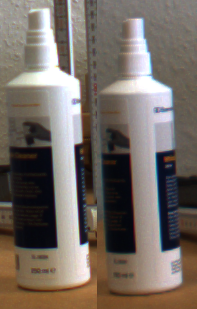
\includegraphics[scale=0.4]{bilder/nonparallal}
	\caption[Stereo Vergr"o"serung]{Stereo Vergr"o"serung}
	\label{fig:vergr}%
\end{figure}

\noindent In \ref{fig:steresene} ist eine Aufnahme der Kameras zu sehen. Durch das genaue Hinsehen erkennt man, dass Referenzpunkte nicht immer auf einer Geraden liegen. Dies ist durch eine Vergr"o"serung, wie in \ref{fig:vergr}, dargestellt. Dies liegt an der Rotation um die $x$-Achse der beiden Kameras. Diese entsteht zum einen durch das nicht exakte Stativ, zum anderen durch die Befestigung der Kameras an diesem. Aufgrund dieser Rotation ist es nicht m"oglich Tiefeninformationen der ganzen Szene zu ermitteln. Um dieses Problem zu beheben, m"ussen die Bilder rektifiziert werden \cite{zbs}. Mittels der Rektifizierung wird die Rotation beider Kameras berechnet und auf den jeweiligen Aufnahmen kompensiert, sodass Referenzpunkte auf einer geraden Linie liegen. In der Epipolargeometrie wird diese Gerade die Epipolarlinie genannt \cite{ocvs} \cite{wepi}. Nach der Rektifizierung sind alle diese Epipolarlinien parallel, was die Suche nach Korrespondenzen vereinfacht. Die Rektifizierung wird in OpenCV mittels der Funktion \textit{stereoRectify} erreicht.

\section{Generierung einer Tiefenkarte} 
\label{sec:gernerierungdep}

Die Tiefenkarte, aus der die Punktewolke generiert wird, wird mit Hilfe des Blockmatching Algorithmus berechnet. Dabei handelt es sich um einen objektorientierten Algorithmus, der zwei gleichgroße Blöcke aus verschiedenen Bildern vergleicht. Es wird ein Bereich im ersten Bild mit allen gleichgroßen Bereichen im zweiten verglichen. Dieser Bereich ist eine \textit{n x m}-Matrix. Der mittlere Quadratische Fehler (MSE) dient als vergleichsmaß, welches sich wie folgt berechnet \cite{HAW}:

\begin{equation}
MSE(x,y,\Delta) = \dfrac{1}{n-m} \sum_{i=-k}^k \sum_{j=-k}^k (|G_{L}(x+i, y+j) - G_{R}(x+i+\Delta, y+j)|^2)
\end{equation}

\noindent $G_{L}$ und $G_{R}$ sind die Bilder als Matrizen in Grauwerten abgespeichert. Der Offset $\Delta$ ist der Indikator f"ur die Sprungweite im zweiten Bild. Nun ist es m"oglich, die Disparit"at $d$ zu bestimmen (die Disparit"at bezeichnet die horizontale Differenz zwischen zwei korrespondierenden Bildpunkten \cite{disp}). Dies beschränkt sich allerdings auf die Bereiche, in der der MSE minimal ist \cite{HAW}:

\begin{equation}
D=\min_{|\Delta|\leq d_{max}} \{MSE(x,y\Delta)\}
\end{equation}

\noindent Durch eine Pixelselektion kann eine Tiefenkarte "uber das ganze Bild erstellt werden.

\begin{figure}%
	\centering
	\subfloat[Stereosystem]{{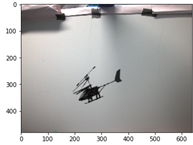
\includegraphics[width=6cm]{bilder/heli_left} }}%
	\qquad
	\subfloat[Szenenaufnahme]{{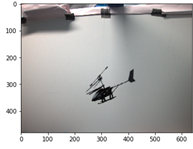
\includegraphics[width=6cm]{bilder/heli_right} }}%
	\caption{Aufnahmen eines Helikopters}%
	\label{fig:stereoheli}%
\end{figure}

\noindent \ref{fig:stereoheli} zeigt Aufnahmen des Helikopters von beiden Kameras. Abbildung \ref{fig:tiefenkarte} zeigt die aus diesen beiden Aufnahmen berechnete Tiefenkarte, auf welcher n"ahe zur Kamera positionierte Objekte dargestellt werden.

\begin{figure}[H]
	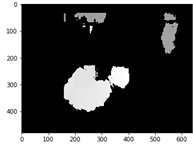
\includegraphics[scale=2.0]{bilder/Tiefenkarte}
	\caption[Tiefenkarte]{Tiefenkarte}
	\label{fig:tiefenkarte}%
\end{figure}

\section{Punktewolken-Generierung} 
\label{sec:pointgen}

Um aus der Tiefenkarte 3D-Koordinaten zu bestimmen, werden zunächst die $x$- und $y$- Werte derjenigen Pixel, die einen Wert größer 0 in der Tiefenkarte aufweisen, mit dem dazugehörigen Disparitätswert $d$ in homogener Schreibweise, d.h. mit einer angehängten 1, in einen Vektor geschrieben. Außerdem werden die Farbwerte dieser Pixel in einer Matrix gespeichert. Der Vektor $(x, y, d, 1)$ wird dann mit der 4 x 4-Perspektiv-Transformations-Matrix $Q$, die durch die Rektifizierung bestimmt wurde multipliziert. Die Matrix $Q$ enthält aktualisierte Informationen über die Brennweite, die Hauptpunktsverschiebung und die Länge der Baseline nach der Rektifizierung. Zum Schluss muss lediglich der Resultatsvektor durch den Wert des letzten Elements geteilt werden, um die Homogenisierung rückgängig zu machen und die gewünschten $x$-, $y$-, und $z$-Koordinaten in kartesicher Form zu erhalten. Diese werden mit den gespeicherten Farbwerten in eine \textit{.ply}-Datei geschrieben, um beispielweise mit CloudCompare anschließend visualisiert werden zu können.\newline
Die Berechnung könnte auch innerhalb einer geschachtelten Schleife, die über sämtliche Pixelwerte iteriert, vorgenommen werden. Der vektorbasierte Ansatz bietet in Python jedoch deutliche Performancevorteile, weshalb die Berechnung auf diese Weise umgesetzt wurde. Das Speichern der Resultate ist optional, es könnte auch direkt mit der Lokalisierung fortgefahren werden, ist jedoch zur Überprüfung der Resultate sehr hilfreich. \ref{fig:cloudresult} zeigt eine Punktewolke, visualisiert mit CloudCompare.

\begin{figure}[H]
	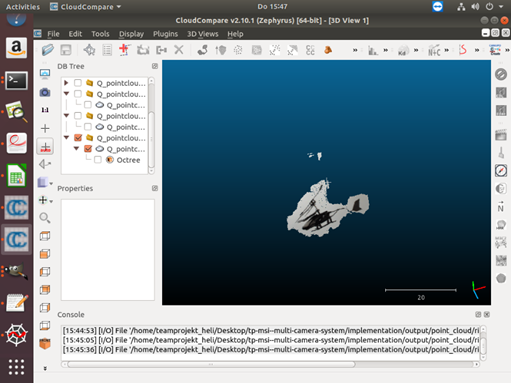
\includegraphics[scale=1.0]{bilder/cloud_result}
	\caption[3D-Punktewolke des Modellhubschraubers vor weißem Hintergrund in CloudCompare]{3D-Punktewolke des Modellhubschraubers vor weißem Hintergrund in CloudCompare}
	\label{fig:cloudresult}%
\end{figure}

\section{Lokalisierung des Helikopters} 
\label{sec:lokalisierung}

\subsection{k-Means}
\label{subsec:kmeans}

Der k-Means Algorithmus ist eine Clusteranalyse, welche verwendet wird, um einen Clustermittelpunkt zu ermitteln. Dafür ist die Clusteranzahl statisch davor zu bestimmen. Da wir unsere Detektion unter Laborbedingungen durchführen kann davon ausgegangen werden, dass es nur ein Cluster gibt, nämlich die Punktewolke des Helikopters. Demnach wird die Clustergröße auf eins gesetzt, um den Mittelpunkt des Helikopters zu ermitteln. {Der Algorithmus partitioniert die Datenpunkte so, dass die summierte Varianz innerhalb jedes Clusters minimiert wird} \cite{KM}.\newline
\noindent Die Problematik in einem lokalen Minimum hängen zu bleiben entfällt, da es nur ein Cluster gibt. Die euklidische Distanz von jedem Punkt zu dem optimalen Clustermittelpunkt wird bestimmt. Der Mittelpunkt des Clusters wird mit folgender Formel berechnet:

\begin{equation}
SSE=\sum_{i=1}^K \sum_{x \in C_i} dist(c_i, x)^{2}
\end{equation}

\noindent SSE (sum of squared error) soll minimiert werden, was zu einem besseren Mittelpunkt des Cluster f"uhrt. Dafür ist es Notwendig $dist$ zu minimieren. Dabei
handelt es sich um den euklidische Abstand von dem Clustermittelpunkt zu dem jeweiligen Punkt. Eine Quadrierung wird vorgenommen um das Vorzeichen zu eliminieren \cite{TUM}. Durch die gegebenen Umstände ist eine Vereinfachung möglich:\newline

\begin{equation}
SSE=\sum_{x \in c_i} dist(c_i, x)^{2}
\end{equation}

\noindent Der Anpassungsschritt, in dem der neue Clustermittelpunkt gewählt wird, wird durch das arithmetisches Mittel ausgerechnet:

\begin{equation}
\mu_k = \dfrac{\sum_{n}x_{n}}{n}
\end{equation}

\begin{figure}[H]
	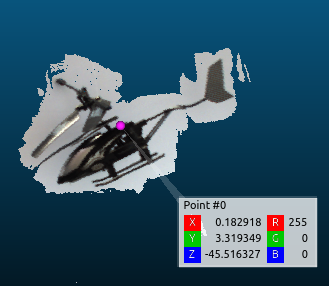
\includegraphics[scale=0.75]{bilder/helicloud}
	\caption[Helikoptercluster]{Helikoptercluster}
	\label{fig:helimeans}%
\end{figure}

\noindent In \ref{fig:helimeans} sieht man den angewandten K-Means Algorithmus auf eine generierte Punktewolke aus unserem Kamerasystem. Gut zu erkennen ist, dass der Mittelpunkt des Helikopterclusters auch in der N"ahe des tats"achliche Mittelpunkt des Helikopters ist.
